\documentclass[a4paper,12pt]{article}
\usepackage{color}
\usepackage{graphicx, gensymb}
\usepackage{amsfonts, cancel, amssymb}
\usepackage{amsmath, amsthm, array, esvect, esint}
\usepackage{typearea, tikz, pgffor, verbatim}
\usetikzlibrary{calc, quotes}
\usepackage[a4paper,left=2cm,right=2cm,top=2cm,bottom=3cm,bindingoffset=5mm]{geometry}
\newcommand\numberthis{\addtocounter{equation}{1}\tag{\theequation}}
\newcommand{\bra}{}
\newcommand{\kom}{}
\newcommand{\brak}{}
\newcommand{\braket}{}
\newcommand{\intx}{}
\newcommand{\intr}{}
\newcommand{\kla}{}
\newcommand{\klam}{}
\newcommand{\klammer}{}
\newcommand{\oper}{}
\newcommand{\tecxt}{}
\newcommand{\Bra}{}
\newcommand{\Ket}{}

\begin{document}

\title{01 Strukturen mit Tikz}
\author{Joachim Schwardt}
\date{\today}
\maketitle

\section{Reziproke Gittervektoren}
Seien die direkten Gittervektoren in einer Matrix $A=(a_{ij})_{ij}:=(\vec{a}_1\vec{a}_2\vec{a}_3)$ angeordnet. Dann erhält man die reziproken Gittervektoren $B:=(\vec{b}_1\vec{b}_2\vec{b}_3)$ komponentenweise aus der Rechenvorschrift
\begin{align*}
b_{ij}&=\frac{2\pi}{\det A}\epsilon_{kli}a_{kj}a_{lj}(=:a_{ij}^\ast)\numberthis\label{Reziproker Operator}\\
B&=\frac{2\pi}{\det A}\kla\left( {\vec{a}_2\times\vec{a}_3,\ \vec{a}_3\times\vec{a}_1,\ \vec{a}_1\times\vec{a}_2} \right)\numberthis\label{Reziproker Operator Matrix}
\end{align*}
Die Determinante von $B$ kann im dreidimensionalen Raum über $\det B=\vec{b}_1\cdot(\vec{b}_2\times\vec{b}_3)$ bestimmt werden:
\begin{align*}
\det B&=\frac{8\pi^3}{(\det A)^3}(\vec{a}_2\times\vec{a}_3)\cdot\kla\left( {(\vec{a}_3\times\vec{a}_1)\times(\vec{a}_1\times\vec{a}_2)} \right)\\
\det B&=\frac{8\pi^3}{(\det A)^3}\epsilon_{abc}\epsilon_{aef}\epsilon_{bgh}\epsilon_{cij}a_{e1}a_{f1}a_{g2}a_{h2}a_{i3}a_{j3}=\\
&=\frac{8\pi^3}{(\det A)^3}\epsilon_{bgh}\epsilon_{cij}a_{e1}a_{f1}a_{g2}a_{h2}a_{i3}a_{j3}(\delta_{be}\delta_{cf}-\delta_{bf}\delta_{ce})=
\end{align*}
Über doppelt vorkommende Indizes wird gemäß der Einsteinschen Summenkonvention summiert. Da das Levi-Civita-Symbol $\epsilon_{kli}$ in drei Dimensionen einem Tensor dritter Stufe entspricht, kann die Rechnung nicht mehr mit Matrizen dargestellt werden. Im zweidimensionalen Fall ergibt sich einfacher $b_{ij}\propto\epsilon_{ki}a_{kj}$. Um zu zeigen, dass $G^{\ast\ast}=G$ gilt, wird die Operation (\ref{Reziproker Operator}) zweimal angewandt. Zudem sei vermerkt, dass $\det a_{ij}=\epsilon_{ijk}a_{i1}a_{j2}a_{k3}$ gilt:
\begin{align*}
c_{ij}&=\frac{2\pi}{\det B}\epsilon_{kli}b_{kj}b_{lj}=\frac{8\pi^3}{(\det A)^2\det B}\epsilon_{kli}\epsilon_{abk}a_{aj}a_{bj}\epsilon_{cdl}a_{cj}a_{dj}=\\
&=\frac{\det A}{\det\epsilon_{kli}a_{kj}a_{lj}}\epsilon_{cdl}a_{aj}a_{bj}a_{cj}a_{dj}(\delta_{la}\delta_{ib}-\delta_{lb}\delta_{ia})=\\
&=\det A\cdot\frac{\epsilon_{cdl}a_{lj}a_{ij}-\epsilon
_{cdl}a_{ij}a_{lj}}{\epsilon_{abc}}a_{cj}a_{dj}
\end{align*} 
\section{Diamantstruktur}
\begin{figure}[h!]
\centering
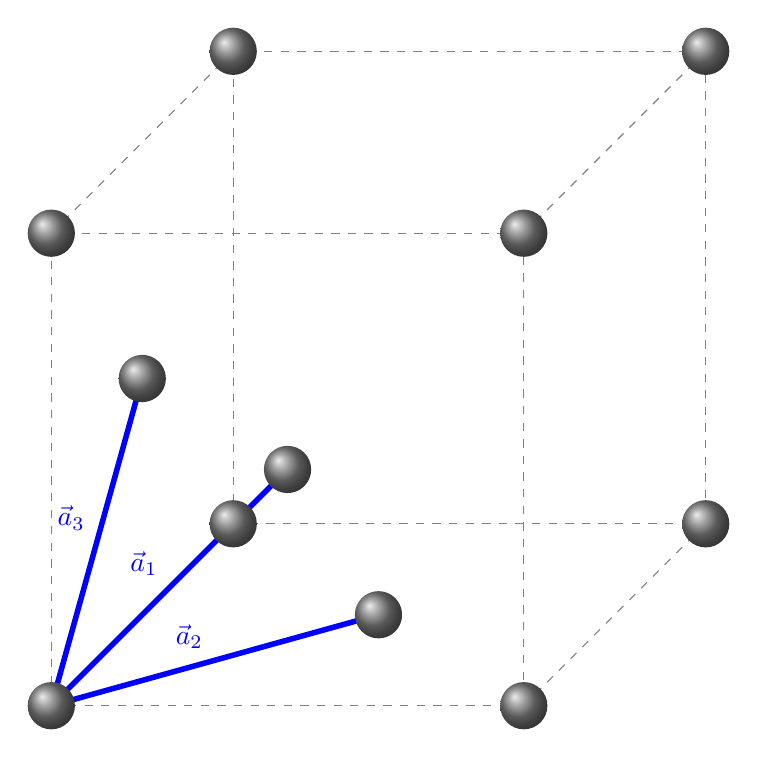
\begin{tikzpicture}[scale=1.5]
\pgfmathsetmacro{\s}{4}
\foreach \z in {0,-\s}{
  \draw[dashed, gray] (0,0,\z) -- (\s,0,\z) -- (\s,\s,\z) -- (0,\s,\z) -- cycle;}
\foreach \x in {0,\s}{
  \foreach \y in {0,\s}{
    \draw[dashed, gray] (\x,\y,0) to (\x,\y,-\s);}}
\foreach \i/\vctr in {1/{0.5*\s,0.5*\s,0},2/{0.5*\s,0,-0.5*\s},3/{0,0.5*\s,-0.5*\s}}{
  \coordinate (a\i) at (\vctr);
  \draw[blue, line width=2] (0,0,0) edge["$\vec{a}_\i$"] (a\i);
  \shade[ball color = gray] (a\i) circle (0.2);}
%\coordinate (a1) at (\s,\s,0);
%\coordinate (a2) at (\s,\s,0);
%\coordinate (a3) at (\s,\s,0);
\foreach \x in {0,\s}{
  \foreach \y in {0,\s}{
    \foreach \z in {0,-\s}{
      \coordinate (\x\y\z) at (\x,\y,\z);
      \shade[ball color = gray] (\x\y\z) circle (0.2);}}}
\end{tikzpicture}
\caption{Diamantstruktur}
\label{figure:Diamantstruktur}
\end{figure}


\end{document}